\documentclass[paper=a4, fontsize=11pt]{scrartcl}
\usepackage[T1]{fontenc}
\usepackage[utf8]{inputenc}
\usepackage{lmodern}
\usepackage{multirow}
\usepackage[table,xcdraw]{xcolor}
\usepackage[spanish]{babel}
\usepackage{cite}
\usepackage{amsmath,amsfonts,amsthm} % Math packages
\usepackage{graphics,graphicx, float} %para incluir imágenes y colocarlas
\usepackage[backref,colorlinks=true,linkcolor=black,urlcolor=blue,citecolor=blue]{hyperref} %Para crear enlaces en el pdf
\usepackage[noabbrev,spanish]{cleveref}
\usepackage{url}
\usepackage[shortlabels]{enumitem}
\usepackage{appendix}
\usepackage{eurosym}
\usepackage{epsfig}
\usepackage{caption}
\usepackage{subcaption}

\renewcommand{\appendixname}{Anexo}
\renewcommand{\appendixtocname}{Anexo}
\renewcommand{\appendixpagename}{Anexo}

\numberwithin{figure}{section} % Number figures within sections (i.e. 1.1, 1.2, 2.1, 2.2 instead of 1, 2, 3, 4)
\numberwithin{table}{section} % Number tables within sections (i.e. 1.1, 1.2, 2.1, 2.2 instead of 1, 2, 3, 4)
\newcommand{\horrule}[1]{\rule{\linewidth}{#1}} % Create horizontal rule command with 1 argument of height

\title{
    \normalfont \normalsize
    \textsc{{\bf Ingeniería de Servidores (2015-2016)} \\ Grado en Ingeniería Informática \\ Universidad de Granada} \\ [25pt] % Your university, school and/or department name(s)
    \horrule{0.5pt} \\[0.4cm] % Thin top horizontal rule
    \huge Memoria Práctica 5 \\ % The assignment title
    \horrule{2pt} \\[0.5cm] % Thick bottom horizontal rule
}
\author{Antonio de la Vega Jiménez }

%*************************************************************


\begin{document}

\maketitle % Muestra el Título
\newpage %inserta un salto de página
\tableofcontents % para generar el índice de contenidos
\listoffigures
\newpage

%*************************************************************

\section{Instalación de servicios y configuraciones}

\subsection{yum}



%***********************************************
%    CUESTIÓN 1
%***********************************************
\subsubsection{Cuestión 1}
\textit{Liste los argumentos de yum necesarios para instalar, buscar y eliminar paquetes.}
\newline

Los argumentos necesarios son: \cite{manyum}
\begin{itemize}
  \item Instalar: \texttt{yum install nombrePaquete}
  \item Buscar: \texttt{yum search nombre}
  \item Eliminar: \texttt{yum remove nombrePaquete o yum erase nombrePaquete}
\end{itemize}



%***********************************************
%    CUESTIÓN 2
%***********************************************
\subsubsection{Cuestión 2}
\textit{Qué ha de hacer para que yum pueda tener acceso a Internet? (Pistas: archivo de configuración en /etc, proxy: stargate.ugr.es:3128). ¿Cómo añadimos un nuevo repositorio?}
\newline

Para conseguir que yum tenga acceso a Internet hay que editar el archivo \textbf{yum.conf} y especificar que se va a acceder a Internet a través de un proxy , como se indica en la figura \ref{fig41}. \cite{centosproxy}

\begin{figure}[H]
    \begin{center}
        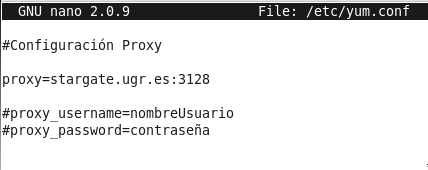
\includegraphics[scale=0.8]{imagenes/img44}
        \caption{Edición del archivo yum.conf para que tenga acceso a internet.}
        \label{fig41}
    \end{center}
\end{figure}


Para añadir un nuevo repositorio en yum, se debe añadir un archivo \textbf{.repo} que contiene la información del repositorio que se quiere añadir al directorio \textbf{/etc/yum.repos.d/} , es importante que el archivo de configuración para cada repositorio incluya el parámetro gpgkey para que la clave publica sea importada automáticamente, en caso de no incluirse, las claves tendrán que ser importadas manualmente. \cite{centosadd}
\subsection{apt}



%***********************************************
%    CUESTIÓN 3
%***********************************************
\subsubsection{Cuestión 3}
\textit{Indique el comando para buscar un paquete en un repositorio y el correspondiente para instalarlo.}
\newline

Los comandos necesarios son: \cite{manapt1} \cite{manapt2}
\begin{itemize}
  \item Buscar: \texttt{apt-cache search expresiónRegular }
  \item Instalar: \texttt{apt-get install nombrePaquete}
\end{itemize}




%***********************************************
%    CUESTIÓN 4
%***********************************************
\subsubsection{Cuestión 4}
\textit{Indiqué qué ha modificado para que apt pueda acceder a los servidores de paquetes a través del proxy. ¿Cómo añadimos un nuevo repositorio?}
\newline

Para que apt pueda acceder a los repositorios a través de un proxy, debemos editar el archivo \textbf{apt.conf} añadiendo una línea en la que se especifica el proxy que se quiere usar. Un ejemplo de la sintaxis que se puede usar para configurar un proxy para http es \cite{aptpx2}  \texttt{Acquire::http::Proxy "http://proxy:8080";}. \cite{aptpx1} 

Existe dos posibilidades para añadir repositorios a apt, mediante el uso de la orden \texttt{add-apt-repository} \cite{aptadd1} o añadiendo la información del repositorio manualmente\cite{aptadd2}. El uso de la orden \texttt{add-apt-repository }es simple, ya que la orden añade automatiamente el repositorio que se le indique. La segunda forma consiste en editar el archivo \textbf{sources.list }añadiendo una linea con el repositorio que se desea añadir, un ejemplo de la sintaxis de esta linea sería:  \texttt{deb http://ftp.debian.org/debian jessie main
}
\subsection{Windows}

\subsection{OpenSuse}


%***********************************************
%    CUESTIÓN OP 1
%***********************************************
\subsubsection{Cuestión opcional 1}
\textit{¿Qué gestores utiliza OpenSuse?}
\newline
 
Los gestores de paquetes usados por OpenSuse son Zypper y Yast, aunque Yast realiza la misma tarea que Zypper pero con interfaz gráfica. \cite{os1} \cite{os2} \cite{os3}





\section{Gestión de los cortafuegos (firewalls)}
%***********************************************
%    CUESTIÓN 5
%***********************************************
\subsection{Cuestión 5}
\textit{¿Qué diferencia hay entre telnet y ssh?}
\newline

Tanto Telnet ( TELecommunication NETwork ) como SSH ( Secure Shell ) son protocolos de acceso remoto, la principal diferencia es la seguridad que ofrecen, Telnet no usa ningún tipo de cifrado en las comunicaciones, por lo que se pueden interceptar todos los datos de la comunicación ( incluyendo contraseñas ), debido a esto , su uso no es muy recomendable. SSH , al contrario que Telnet, si es un protocolo seguro, ya que todas las comunicaciones van cifradas. \cite{sshtle}





%***********************************************
%    CUESTIÓN 6
%***********************************************
\subsection{Cuestión 6}
\textit{¿Para qué sirve la opción -X? Ejecute remotamente, es decir, desde la máquina anfitriona (si tiene Linux) o desde la otra máquina virtual, el comando gedit en una sesión abierta con ssh. ¿Qué ocurre?}
\newline

La opción -X de SSH sirve para que la aplicación se ejecute en el servidor remoto, pero la interfaz gráfica se visualice en el ordenador local ( X11 forwarding ). \cite{sshx} Al ejecutar gedit desde la terminal SSH, se muestra la aplicación como si se estuviese ejecutando en nuestro ordenador, pero en la ventana se indica que se esta ejecutando en otro ordenador ( on Ubuntu) figura \ref{fig1}. En la figura \ref{fig57} se muestra que en la en la máquina local no se esta ejecutando ningún proceso de gedit mientras que en la remota si.

\begin{figure}[H]
    \begin{center}
    \advance\leftskip-2.5cm
        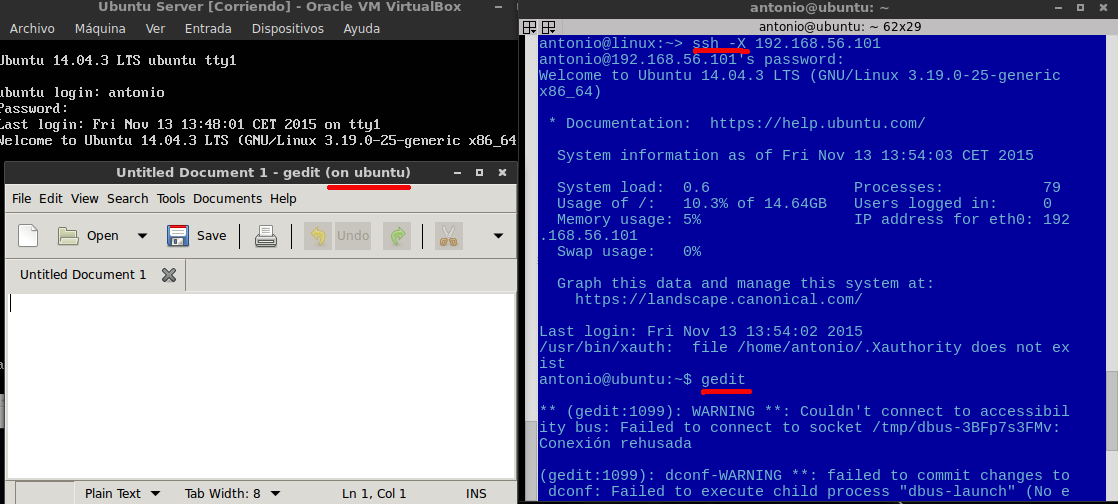
\includegraphics[scale=0.5]{imagenes/img1}
        \caption{En esta imagen se muestra el resultado de ejecutar SSH con la opción -X. Como se puede ver, en la aplicación gedit se indica que la aplicación no esta siendo ejecutada en la máquina local, si no que se esta ejecutando en Ubuntu.}
        \label{fig1}
    \end{center}
\end{figure}


\begin{figure}[H]
    \begin{center}
    \advance\leftskip-2.5cm
        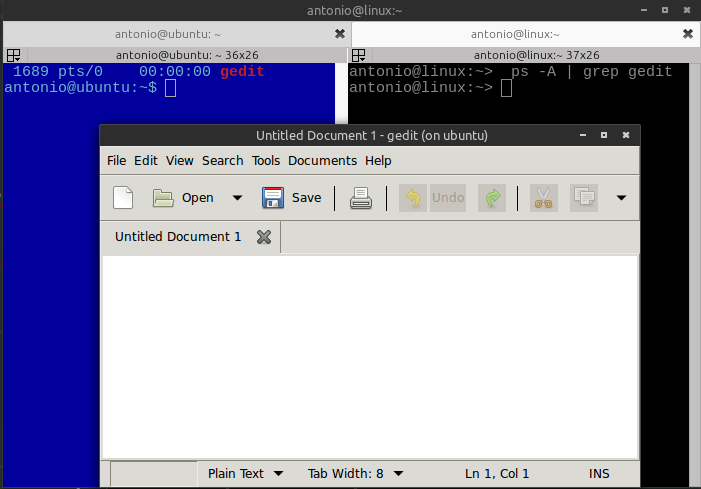
\includegraphics[scale=0.5]{imagenes/img60}
        \caption{Máquina remota ( azul ) en la que se esta ejecutando gedit, junto a la máquina local (negra) en la que aunque se muestra la interfaz gráfica, no se esta ejecutando gedit..}
        \label{fig57}
    \end{center}
\end{figure}


%***********************************************
%    CUESTIÓN 7
%***********************************************
\subsection{Cuestión 7}
\textit{Muestre la secuencia de comandos y las modificaciones a los archivos correspondientes para permitir acceder a la consola remota sin introducir la contraseña. (Pistas: ssh-keygen, ssh-copy-id).}
\newline

El proceso para permitir acceder a la consola sin introducir la contraseña consta de dos pasos: En primer lugar debemos crear una clave RSA y una carpeta para guardarla (en caso de que no exista ) , para ello hacemos uso de los comandos mostrados en la figura \ref{fig2}. En segundo lugar debemos transferir la clave RSA que acabamos de crear al servidor remoto como se puede ver en la figura \ref{fig3}, por último realizaremos una conexión SSH a la máquina remota y en caso de que no se nos pida una contraseña habremos verificado que la configuración se ha realizado correctamente ( figura \ref{fig4}). \cite{passssh}

\begin{figure}[H]
    \begin{center}
        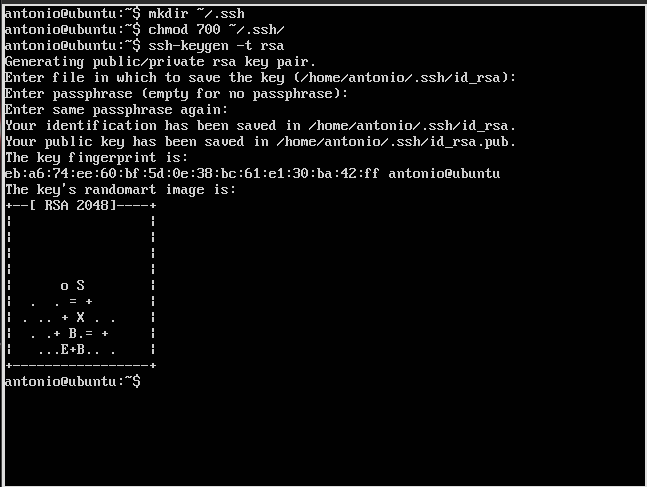
\includegraphics[scale=0.45]{imagenes/img2}
        \caption{Secuencia de comandos necesaria para generar la clave RSA y la carpeta que guarda la clave.}
        \label{fig2}
    \end{center}
\end{figure}

\begin{figure}[H]
    \begin{center}
        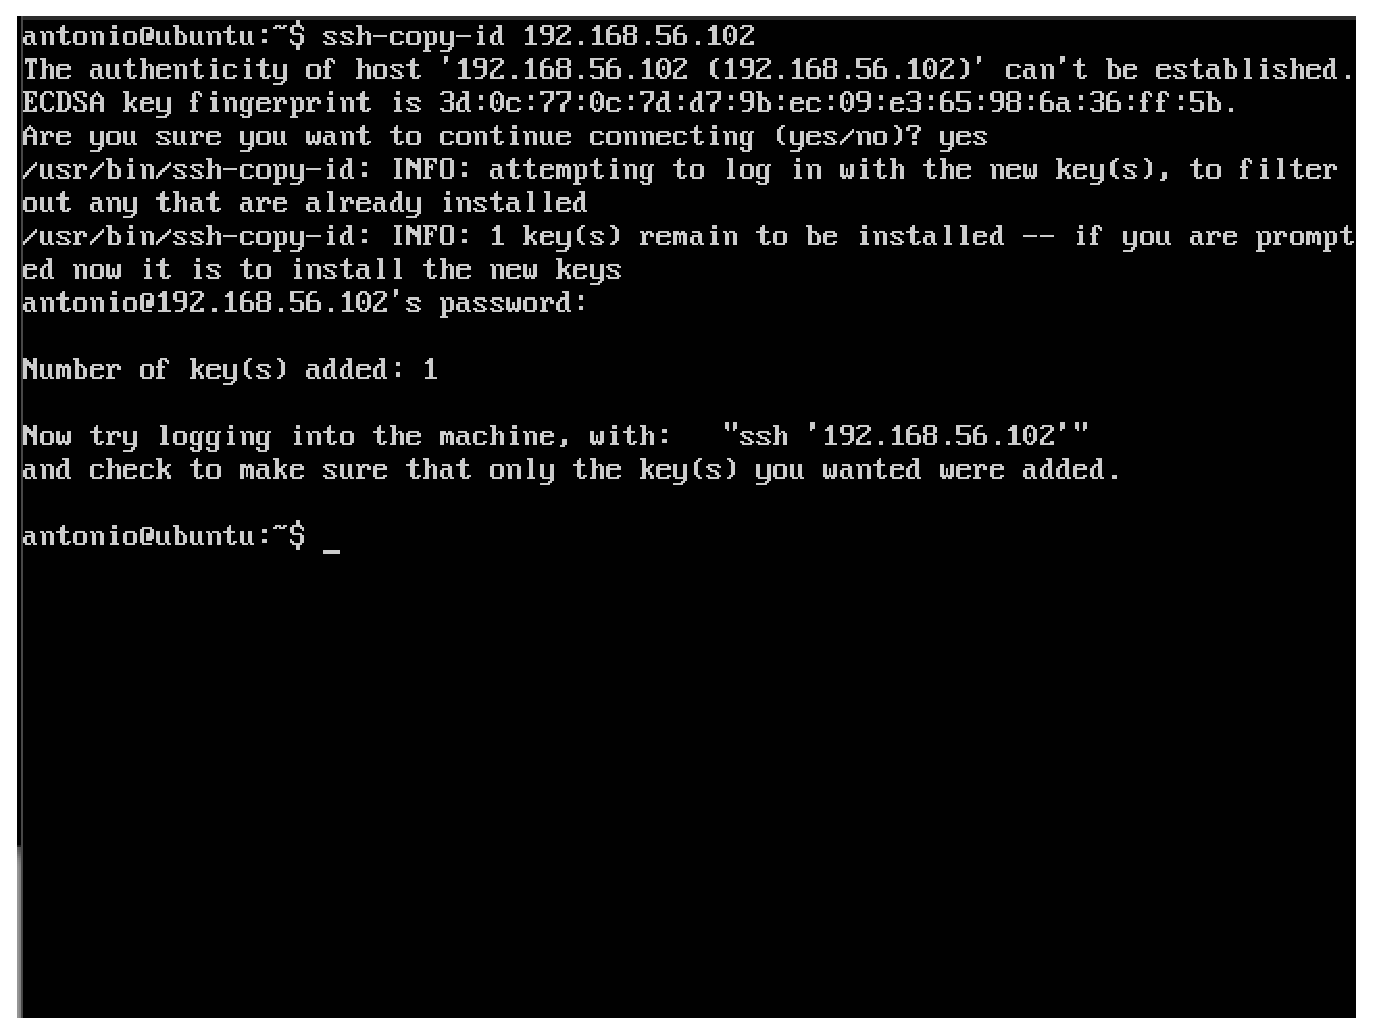
\includegraphics[scale=0.45]{imagenes/img3}
        \caption{Comando para el traspaso de la clave de la máquina local a la máquina remota.}
        \label{fig3}
    \end{center}
\end{figure}

\begin{figure}[H]
    \begin{center}
        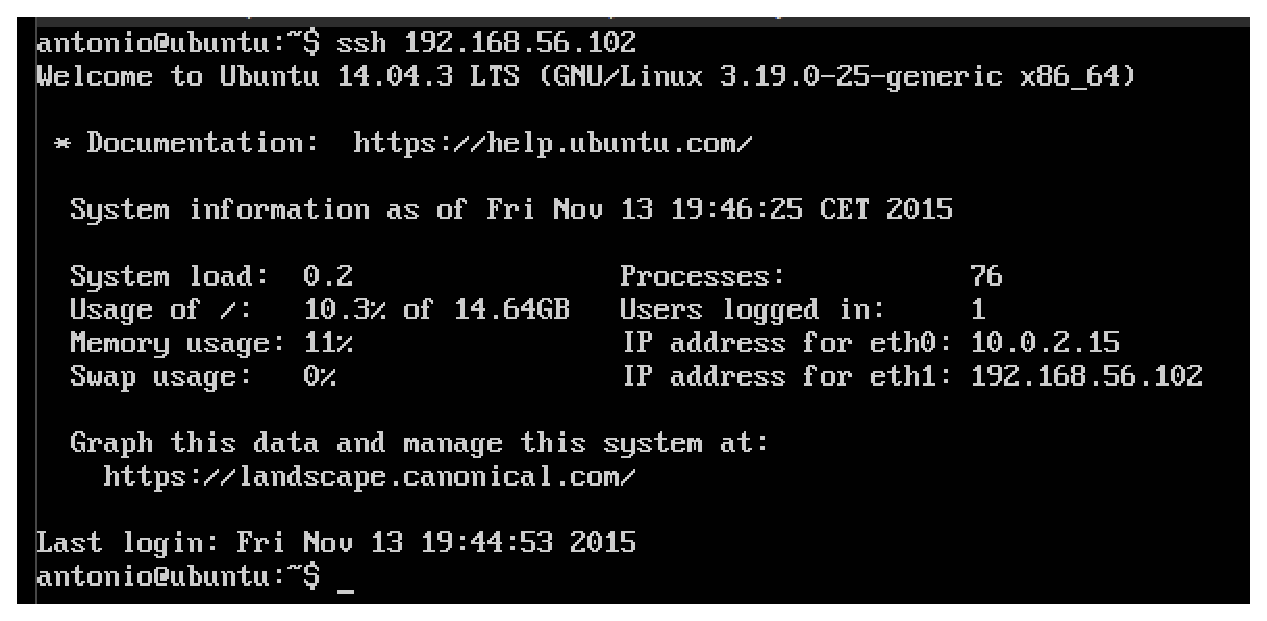
\includegraphics[scale=0.5]{imagenes/img4}
        \caption{Comprobación de que podemos realizar una conexión SSH sin necesidad de introducir contraseña.}
        \label{fig4}
    \end{center}
\end{figure}







%***********************************************
%    CUESTIÓN 8
%***********************************************
\subsection{Cuestión 8}
\textit{¿Qué archivo es el que contiene la configuración de sshd? ¿Qué parámetro hay que modificar para evitar que el usuario root acceda? Cambie el puerto por defecto y compruebe que puede acceder.}
\newline

La configuración de sshd ( SSH daemon ) se encuentra en el archivo sshd\_config que se encuentra en /etc/ssh/sshd\_config. El parámetro que hay que modificar para que root no pueda acceder es PermitRootLogin y establecerlo a no, para cambiar el puerto se debe modificar el parámetro Port, tras realizar estas modificaciones, es necesario reiniciar SSH para que tengan efecto, esto se pude realizar mediante la orden \texttt{sudo service ssh restart} ( Ver configuración en las figuras \ref{fig5} \ref{fig6} y el funcionamiento tras cambiar el puerto en la figura \ref{fig7} y la imposibilidad de entrar como root en la figura \ref{fig8} ) \cite{sshd}

\begin{figure}[H]
    \begin{center}
        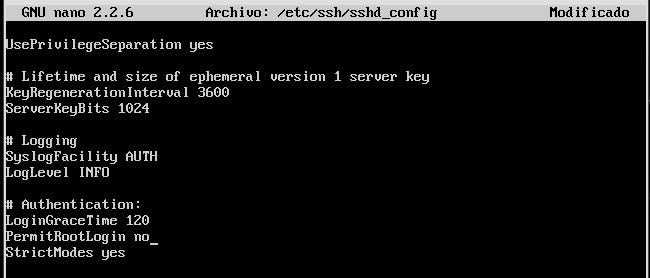
\includegraphics[scale=0.6]{imagenes/img5}
        \caption{Configuracion par que root no pueda acceder (PermitRootLogin no).}
        \label{fig5}
    \end{center}
\end{figure}

\begin{figure}[H]
    \begin{center}
        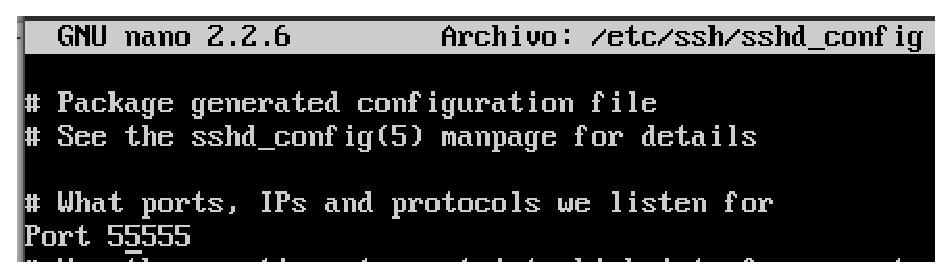
\includegraphics[scale=0.7]{imagenes/img7}
        \caption{Cambio del puerto 22 establecido por defecto en SSH al puerto 55555.}
        \label{fig6}
    \end{center}
\end{figure}

\begin{figure}[H]
    \begin{center}
        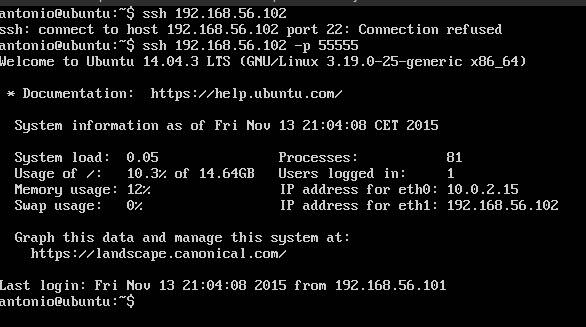
\includegraphics[scale=0.6]{imagenes/img6}
        \caption{Comprobación de que el nuevo puerto SSH es el puerto 55555.}
        \label{fig7}
    \end{center}
\end{figure}

\begin{figure}[H]
    \begin{center}
        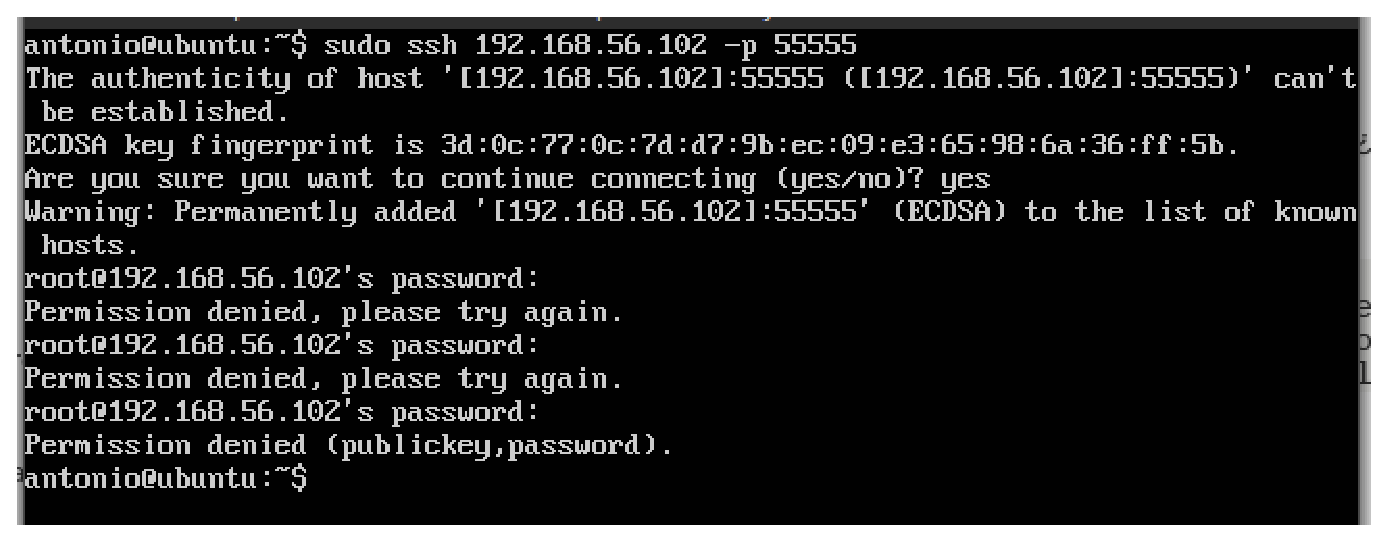
\includegraphics[scale=0.6]{imagenes/img8}
        \caption{Comprobación de que no es posible acceder con el usuario root.}
        \label{fig8}
    \end{center}
\end{figure}






%***********************************************
%    CUESTIÓN 9
%***********************************************
\subsection{Cuestión 9}
\textit{Indique si es necesario reiniciar el servicio ¿Cómo se reinicia un servicio en Ubuntu? ¿y en CentOS? Muestre la secuencia de comandos para hacerlo.}
\newline

En ubuntu un servicio se puede reiniciar de dos formas,de la forma tradicional \newline
 \texttt{ /etc/init.d/nombreServicio restart } o de haciendo uso de  Upstart \newline
 \texttt{service nombreServicio start}. \cite{rest1} En CentOS( y RedHat ) los servicios se reinician mediante las ordenes anteriores o la orden
 \texttt{systemctl restart nombre.service}. \cite{rest2}






\subsubsection{Utilidades: screen y terminator}
%***********************************************
%    CUESTIÓN OP 2
%***********************************************
\paragraph{Cuestión opcional 2}
\textit{Instale y pruebe terminator. Con screen, pruebe su funcionamiento dejando sesiones ssh abiertas en el servidor y recuperándolas posteriormente.}
\newline

Para instalar terminator en OpenSuse se puede realizar como se indica en la figura \ref{fig10} . Para mostrar el funcionamiento de screen he ejecutado \texttt{screen} (figura \ref{fig12}, una vez ahí he ejecutado la orden top (figura \ref{fig13}) y mediante la combinación \texttt{Ctrl+a+d} me he desconectado de la ejecución de top (figura \ref{fig14} y para terminar haciendo uso de la orden \texttt{screen -r } he vuelto a conectarme con la terminal que estaba ejecutando top (figura \ref{fig15}), con esto se muestra que aunque pierdas la conexión con una terminal, luego es posible recuperarla sin ningún tipo de problema. Este proceso se muestra en la figura \ref{fig16}


\begin{figure}[H]
    \centering
    \begin{subfigure}[b]{0.55\textwidth}
        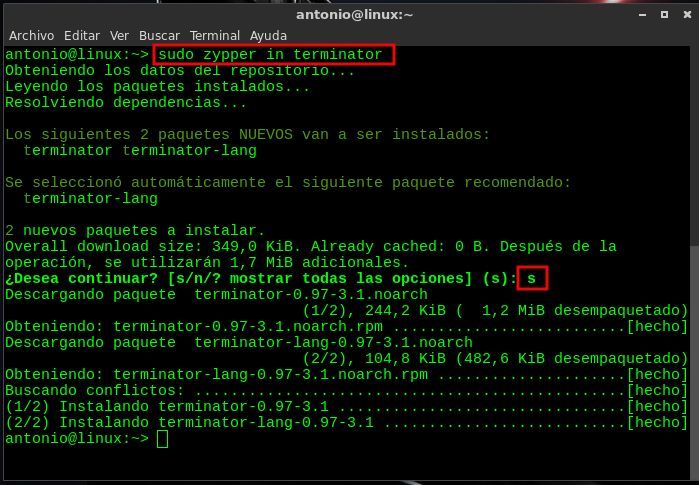
\includegraphics[width=\textwidth]{imagenes/img11}
        \caption{Comando para la instalación de terminator.}
        \label{fig10}
    \end{subfigure}
    \begin{subfigure}[b]{0.4\textwidth}
        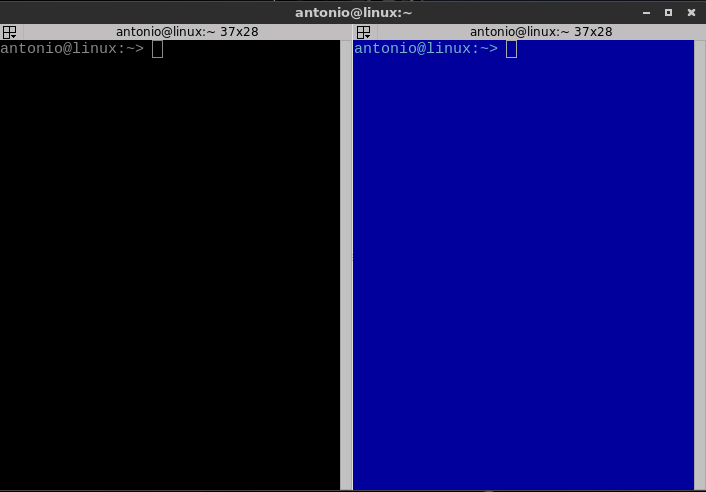
\includegraphics[width=\textwidth]{imagenes/img10}
        \caption{Muestra de dos de las características mas importantes de terminator,dividir la terminal y la creación distintos perfiles.}
        \label{fig11}
    \end{subfigure}
    \caption{Terminator}
\end{figure}



\begin{figure}[H] 
  \begin{subfigure}[b]{0.5\linewidth}
    \centering
    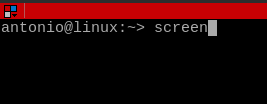
\includegraphics[width=0.75\linewidth]{imagenes/img12} 
    \caption{Ejecución de screen.} 
    \label{fig12} 
    \vspace{4ex}
  \end{subfigure}%% 
  \begin{subfigure}[b]{0.5\linewidth}
    \centering
    
\includegraphics[width=0.75\linewidth]{imagenes/img13} 
    \caption{Ejecución de top.} 
    \label{fig13} 
    \vspace{4ex}
  \end{subfigure} 
  \begin{subfigure}[b]{0.5\linewidth}
    \centering
    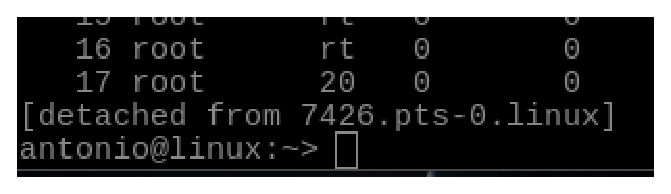
\includegraphics[width=0.75\linewidth]{imagenes/img14} 
    \caption{Desconexión de la terminal con top.} 
    \label{fig14} 
  \end{subfigure}%%
  \begin{subfigure}[b]{0.5\linewidth}
    \centering
    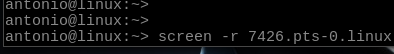
\includegraphics[width=0.75\linewidth]{imagenes/img15} 
    \caption{Reconexión con top.} 
    \label{fig15} 
  \end{subfigure} 
  \caption{screen}
  \label{fig16} 
\end{figure}






\subsubsection{Un poco de seguridad: fail2ban}
%***********************************************
%    CUESTIÓN OP 3
%***********************************************
\paragraph{Cuestión opcional 3}
\textit{Instale el servicio y pruebe su funcionamiento.}


\section{Instalación del servicio de acceso remoto a la consola (Secure Shell)}


\section{Administración remota de windows}


\section{Instalación de un servidor Web básico}

\subsection{Instalación de Apache + MySQL (o MariaDB) + PHP (o Python) en Linux (LAMP)}





%***********************************************
%    CUESTIÓN 10
%***********************************************
\subsubsection{Cuestión 10}
\textit{Muestre los comandos que ha utilizado en Ubuntu Server y en CentOS (aunque en este último puede utilizar la GUI, en tal caso, realice capturas de pantalla)}
\newline

Para la instalación de LAMP en Ubuntu, he instalado los paquetes de  PHP, MySql y Apache de forma individual, haciendo uso de los siguientes comandos: \cite{l1 ,l2 ,l3} \newline

\hskip3.5cm \texttt{sudo apt-get install apache2 }

\hskip3.5cm \texttt{sudo apt-get install mysql-server }

\hskip3.5cm \texttt{sudo apt-get install php5 libapache2-mod-php5}

El funcionamiento del servidor se puede ver en la figura \ref{fig17}

\begin{figure}[H]
    \begin{center}
        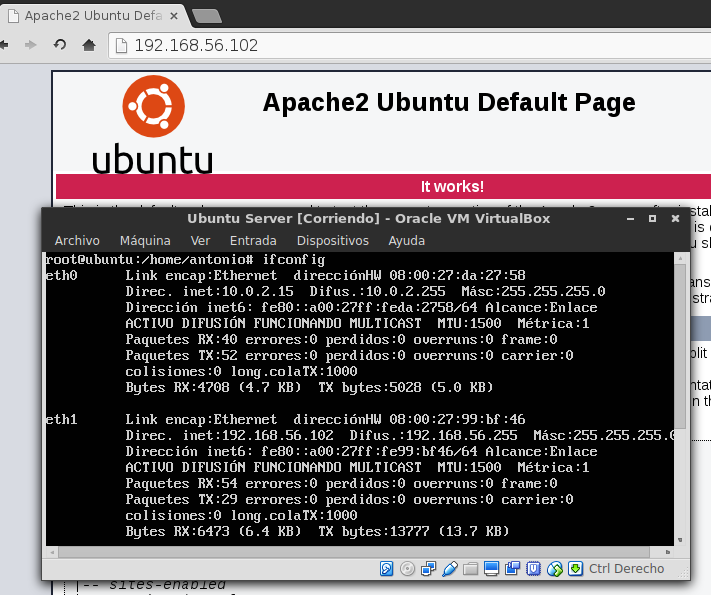
\includegraphics[scale=0.6]{imagenes/img17}
        \caption{Ejecución del servidor LAMP.}
        \label{fig17}
    \end{center}
\end{figure}

Para la instalación de LAMP en CentOS, en primer lugar abrimos el gestor de software como se indica en la figura \ref{fig18}, una vez hay buscamos e instalamos los paquetes \textbf{\texttt{httpd}} (apache), \textbf{\texttt{php}}, \textbf{\texttt{mysql-server}} y opcionalmente \textbf{\texttt{php-mysql}} (para usar MySQL desde PHP ) \cite{l4}. En la figura \ref{fig19} se muestra el servidor en funcionamiento.

\begin{figure}[H]
    \begin{center}
        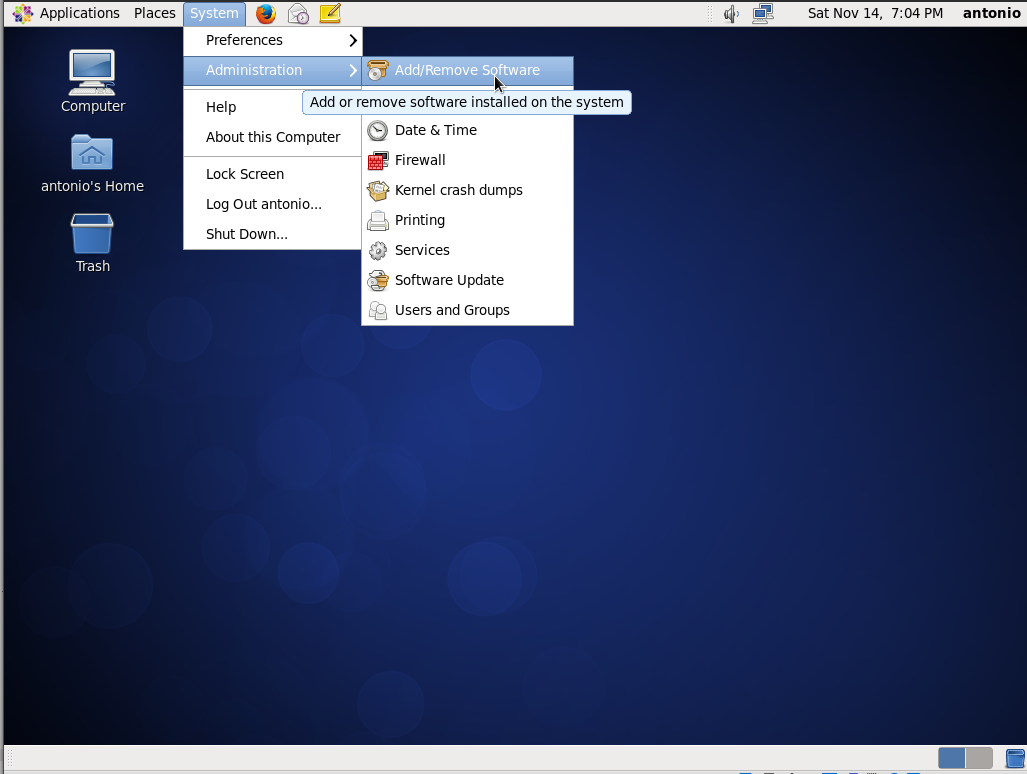
\includegraphics[scale=0.31]{imagenes/img18}
        \caption{Acceso al gestor de software en Centos.}
        \label{fig18}
    \end{center}
\end{figure}

\begin{figure}[H]
    \begin{center}
        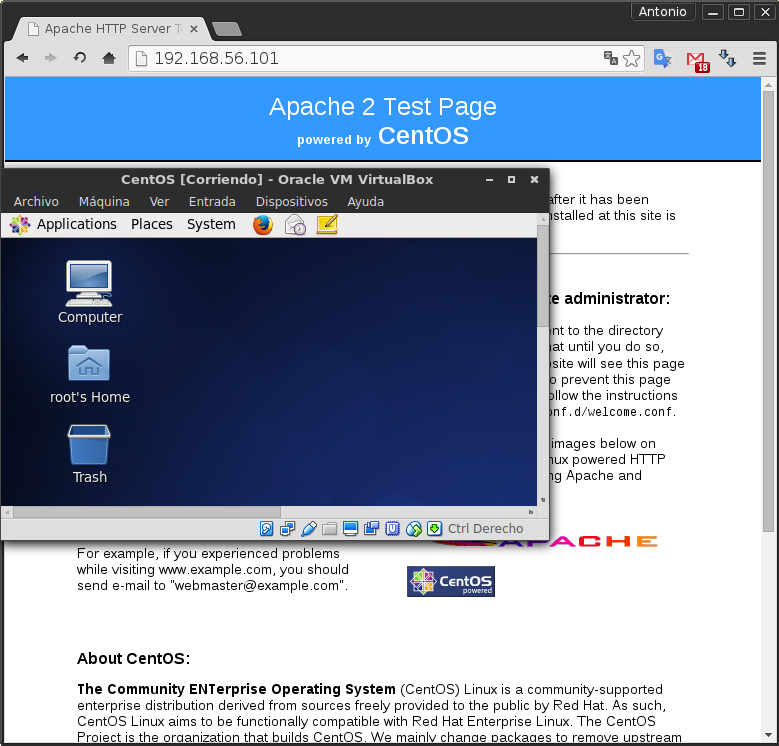
\includegraphics[scale=0.35]{imagenes/img19}
        \caption{Servidor Apache en CentOS.}
        \label{fig19}
    \end{center}
\end{figure}






%***********************************************
%    CUESTIÓN 11
%***********************************************
\subsubsection{Cuestión 11}
\textit{Enumere otros servidores web y las páginas de sus proyectos (mínimo 3 sin considerar Apache, IIS ni nginx).}
\newline

Algunos servidores web son:
\begin{itemize}
  \item \textbf{Abyss Web Server: } \url{www.aprelium.com/abyssws/}
  \item \textbf{Hiawatha: } \url{www.hiawatha-webserver.org}
  \item \textbf{Lighttpd: } \url{www.lighttpd.net}
  \item \textbf{Cherokee: } \url{www.cherokee-project.com}
\end{itemize}






\subsection{Windows: IIS}
%***********************************************
%    CUESTIÓN 12
%***********************************************
\subsubsection{Cuestión 12}
\textit{Compruebe que el servicio está funcionando accediendo a la MV a través de la anfitriona.}
\newline

Tras realizar el proceso indicado en el punto 3.4.2 de la guía de la práctica para comprobar podemos  el funcionamiento de IIS introduciendo la IP del servidor en el navegador del host y ver que se accede a un web de IIS predeterminada, como se muestra en la figura \ref{fig20}.

\begin{figure}[H]
    \begin{center}
        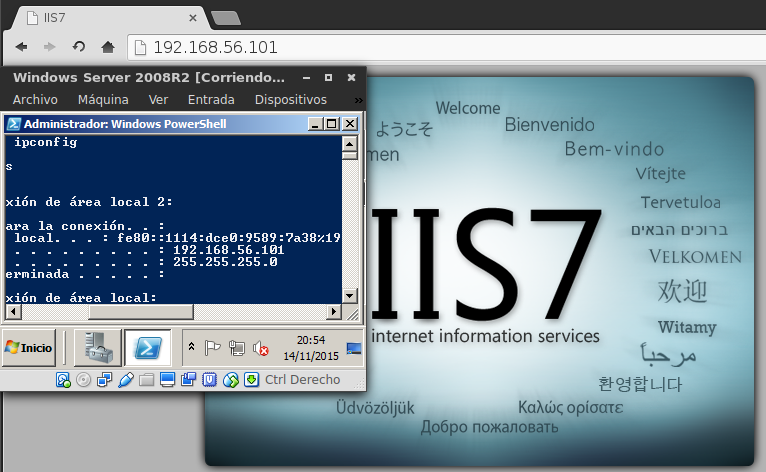
\includegraphics[scale=0.5]{imagenes/img20}
        \caption{Muestra de que IIS se está ejecutando correctamente.}
        \label{fig20}
    \end{center}
\end{figure}

\subsection{Windows y otros servidores web}





\subsection{Java Servlets}
%***********************************************
%    CUESTIÓN OP 4
%***********************************************
\subsubsection{Cuestión opcional 4}
\textit{Realice la instalación de uno de estos dos “web containers” y pruebe su ejecución.}
\newline

He llevado a cabo la instalación de Tomcat, haciendo uso de la orden mostrada en la figura \ref{tc1}, luego para comprobar que Tomcat se esta ejecutando correctamente, he abierto un navegador web en la máquina local y he accedido a Tomcat (figura \ref{tc2} haciendo uso de la IP de la máquina remota y del puerto 8080, que es el puerto por defecto para Tomcat. \cite{tomcat}

\begin{figure}[H]
    \begin{center}
        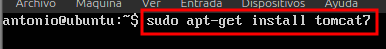
\includegraphics[scale=0.8]{imagenes/tc1}
        \caption{Comando para la instalación de Tomcat.}
        \label{tc1}
    \end{center}
\end{figure}

\begin{figure}[H]
    \begin{center}
        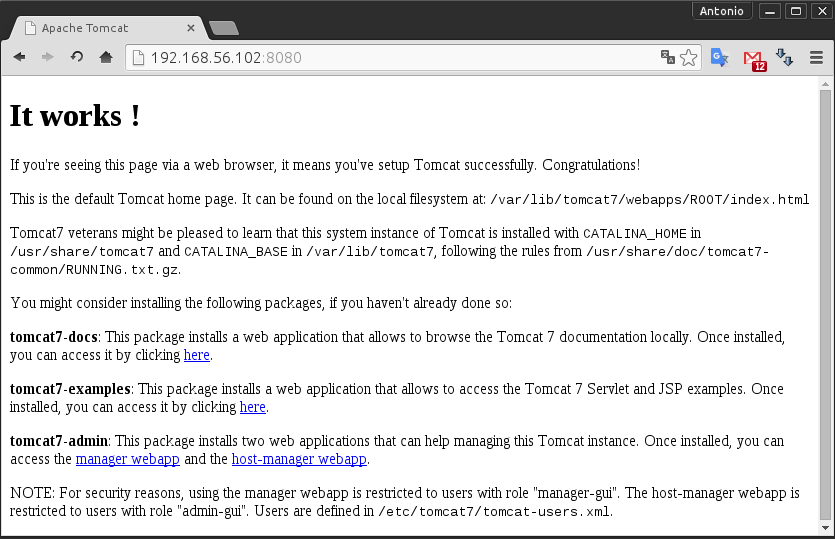
\includegraphics[scale=0.5]{imagenes/tc2}
        \caption{Página mostrada por defecto al acceder al servidor Tomcat.}
        \label{tc2}
    \end{center}
\end{figure}




\subsection{Otro tipo de Bases de datos}
%***********************************************
%    CUESTIÓN OP 5
%***********************************************
\subsubsection{Cuestión opcional 5}
\textit{Realice la instalación de MongoDB en alguna de sus máquinas virtuales. Cree una colección de documentos y haga una consulta sobre ellos. ( http://docs.mongodb.org/manual/installation/ )}







\section{Manteniendo los servicios actualizados}
%***********************************************
%    CUESTIÓN 13
%***********************************************
\subsection{Cuestión 13}
\textit{Muestre un ejemplo de uso del comando patch(p.ej. http://fedoraproject.org/wiki/VMWare)}
\newline

Para realizar esta cuestión he creado dos archivos que contienen nombres, simulando lo que podrían ser archivos de código, haciendo uso de la orden \texttt{diff} \cite{diff} he creado un archivo que contiene las diferencias entre las dos versiones, es decir, un parche, luego haciendo uso de la orden \texttt{patch} \cite{patch}, que sirve para aplicar parches, y del archivo creado anteriormente con los cambios, he ``parcheado'' la versión antigua del archivo, de modo que ahora  la versión antigua contiene las lineas añadidas en la versión nueva. Los archivos y el proceso para generar y aplicar el parche , se puede ver en las figuras \ref{fig60} y \ref{fig61}.


\begin{figure}[H]
    \begin{center}
        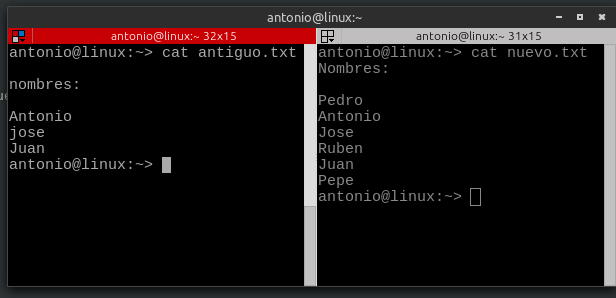
\includegraphics[scale=0.5]{imagenes/img61}
        \caption{Contenido de los archivos usados para hacer la prueba de \texttt{patch}.}
        \label{fig60}
    \end{center}
\end{figure}

\begin{figure}[H]
    \begin{center}
        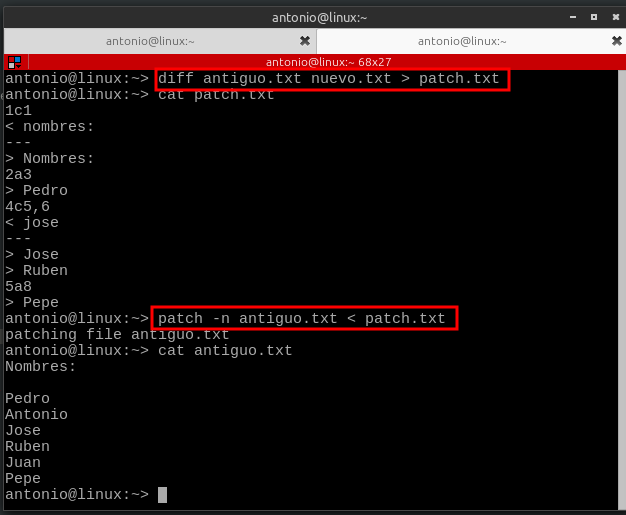
\includegraphics[scale=0.5]{imagenes/img62}
        \caption{En esta imagen se muestra, en primer lugar, el uso del comando \texttt{diff}, que sirve para detectar las diferencias entre dos archivos, luego se muestras, cual es el contenido del archivo creado con \texttt{diff}, tras esto se puede ver el uso del comando \texttt{patch}, que haciendo uso del archivo con las diferencias, actualiza el archivo antiguo y por último se puede observar como queda actualizado el archivo antiguo.}
        \label{fig61}
    \end{center}
\end{figure}

\section{Administración web}
%***********************************************
%    CUESTIÓN 14
%***********************************************
\subsection{Cuestión 14}
\textit{Realice la instalación de esta aplicación (webmin) y pruebe a modificar algún parámetro de algún servicio. Muestre las capturas de pantalla pertinentes así como el proceso de instalación.}
\newline

La instalacón de Webmin se realiza mediante los pasos indicados en la figura \ref{fig21}. \cite{webmin}
\begin{figure}[H]
    \centering
    \begin{subfigure}[b]{1\textwidth}
        
\includegraphics[width=\textwidth]{imagenes/img22}
        \caption{Instalación de dependencias para webmin.}
    \end{subfigure}
    
        \begin{subfigure}[b]{1\textwidth}
        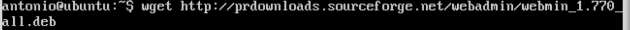
\includegraphics[width=\textwidth]{imagenes/img23}
        \caption{Descarga de el paquete .ded de webmin.}
    \end{subfigure}
    
        \begin{subfigure}[b]{1\textwidth}
        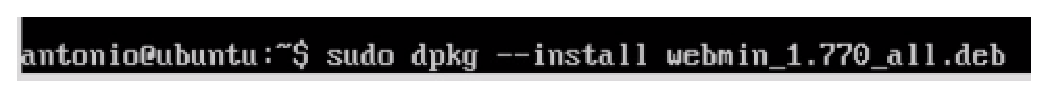
\includegraphics[width=\textwidth]{imagenes/img24}
        \caption{Instalación de webmin.}
    \end{subfigure}
    \caption{Instalación Webmin}
     \label{fig21} 
\end{figure}

Para realizar una prueba de webmin he accedido a webmin desde el ordenador local ( figura \ref{fig22} ), luego me he dirigido al apartado del servicio SSH ( figura \ref{fig23} ) y he lo he modificado para que no se puedan realizar conexiones SSH con el usuario ``antonio'' ( figuras \ref{fig24} \ref{fig25}).



\begin{figure}[H]
    \centering
    \begin{subfigure}[b]{0.7\textwidth}
        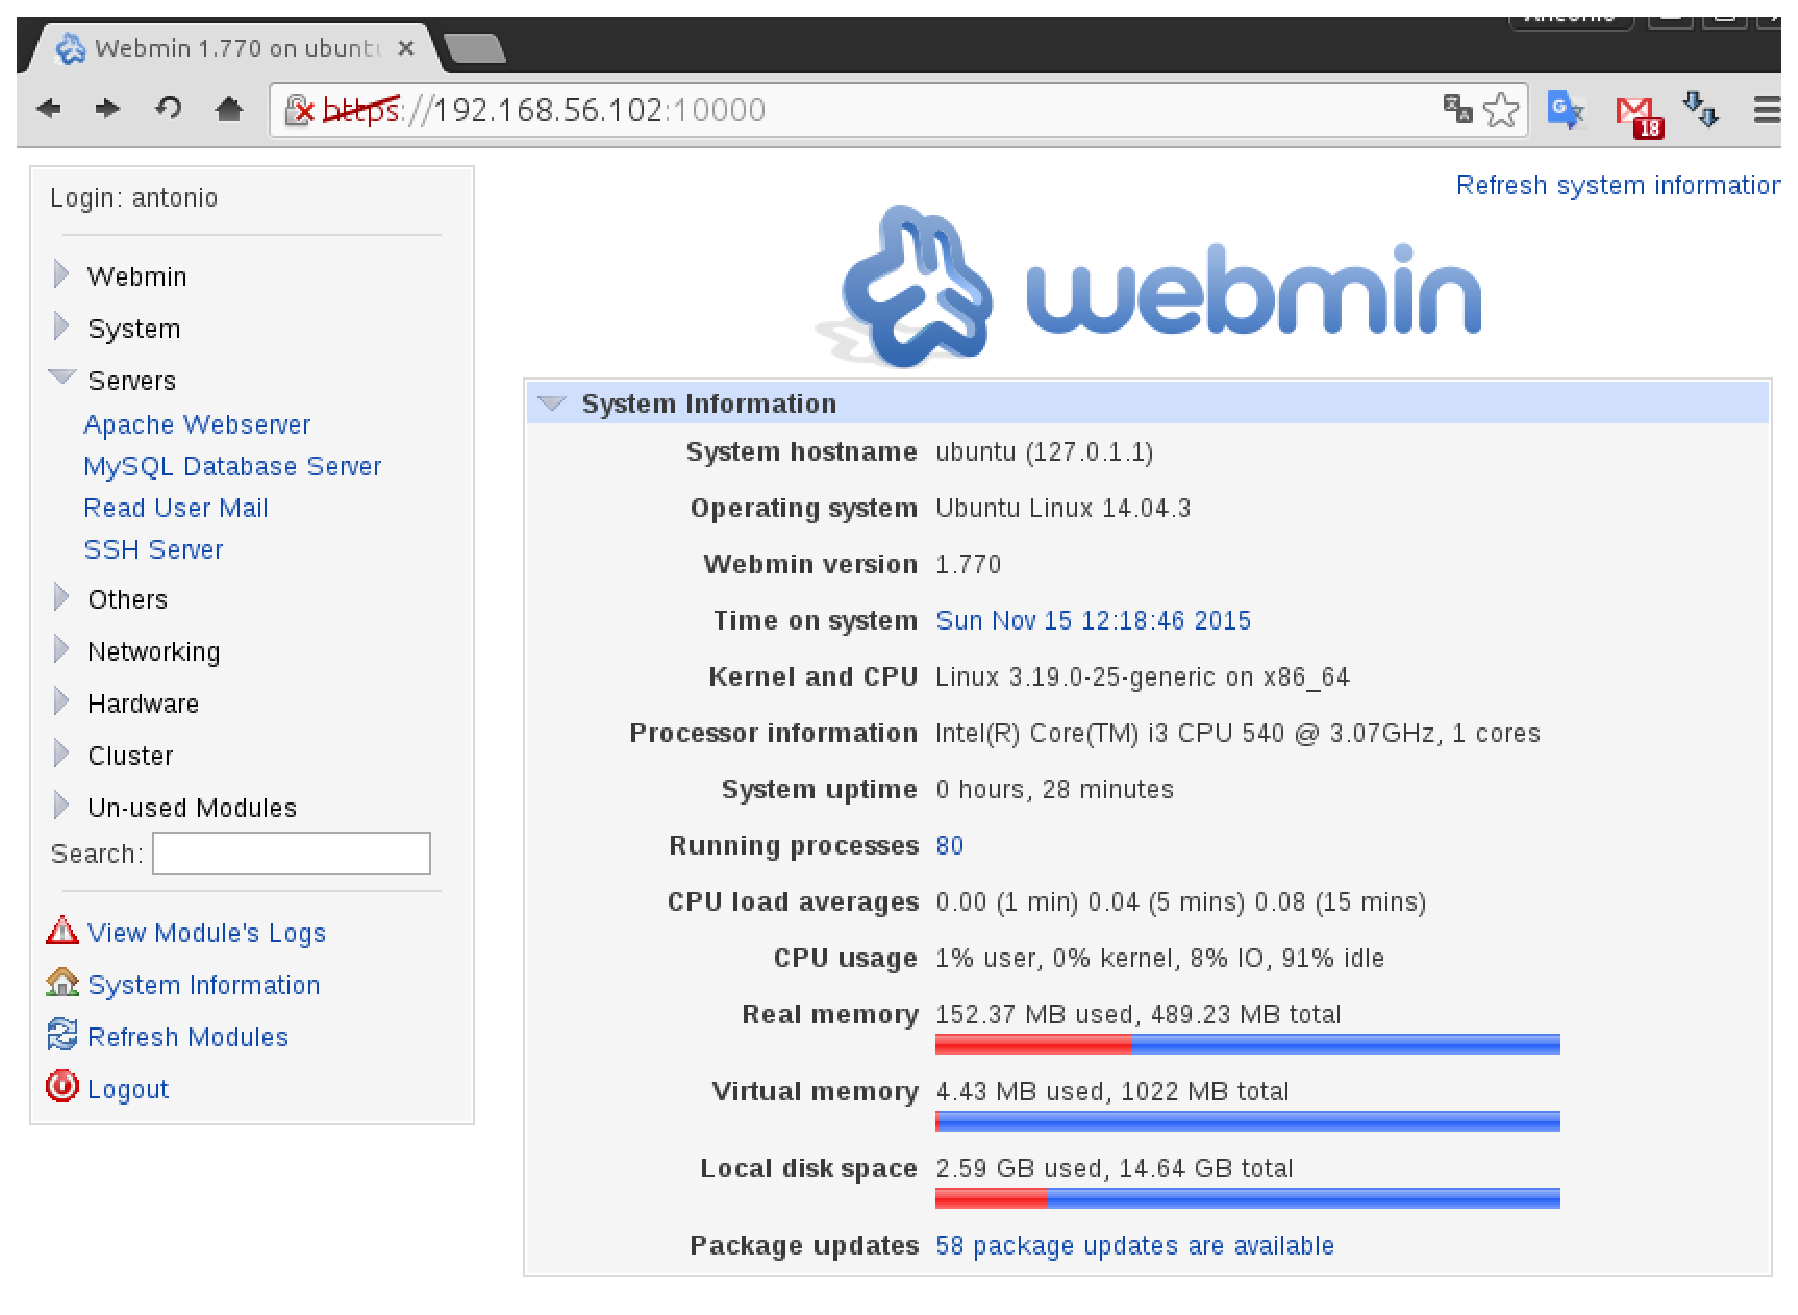
\includegraphics[width=\textwidth]{imagenes/img25}
    \caption{Pantalla inicial webmin.} 
    \label{fig22} 
    \end{subfigure}
    
        \begin{subfigure}[b]{0.7\textwidth}
        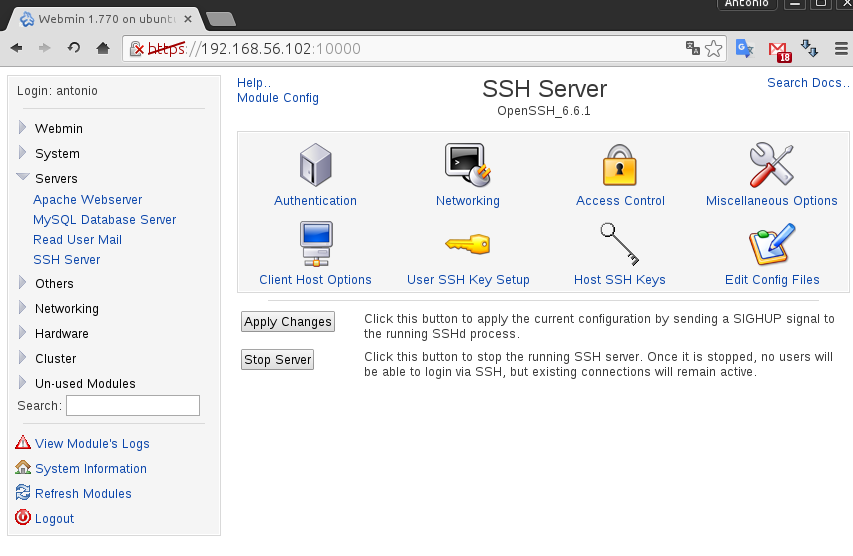
\includegraphics[width=\textwidth]{imagenes/img26}
    \caption{Panel configuración SSH.} 
    \label{fig23} 
    \end{subfigure}
        \caption{Ejemplo de uso de webmin  (Parte 1 ).}  
\end{figure}

    \begin{figure}[H]
    \centering
     \begin{subfigure}[b]{0.7\textwidth}
        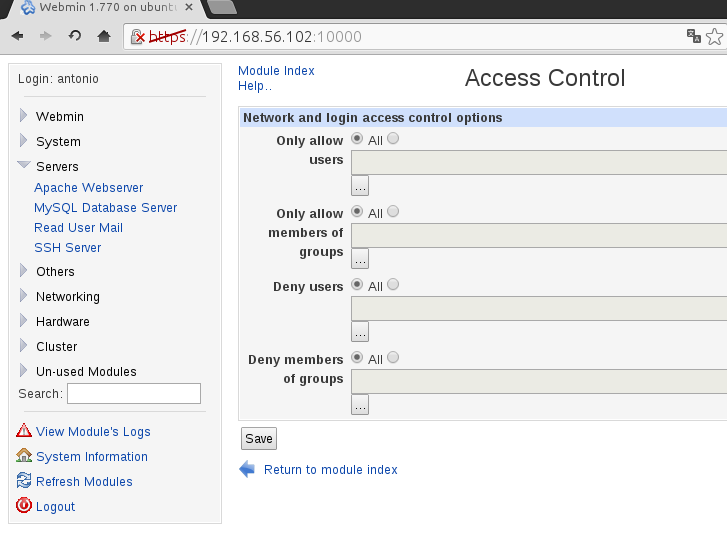
\includegraphics[width=\textwidth]{imagenes/img27}
    \caption{Panel control de acceso SSH.} 
    \label{fig24} 
    \end{subfigure}
    
    \begin{subfigure}[b]{0.7\textwidth}
       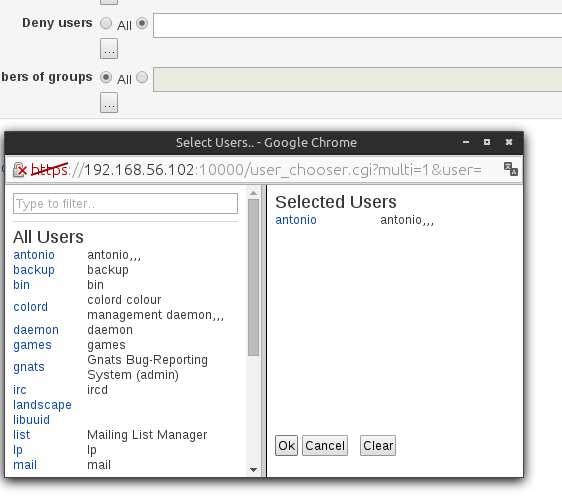
\includegraphics[width=\textwidth]{imagenes/img28}
    \caption{Menú para seleccionar usuarios que no puede usar SSH .} 
    \label{fig25} 
    \end{subfigure}
    \caption{Ejemplo de uso de webmin (Parte 2 ).}  

\end{figure}






%***********************************************
%    CUESTIÓN 15
%***********************************************
\subsection{Cuestión 15}
\textit{Instale phpMyAdmin, indique cómo lo ha realizado y muestre algunas capturas de pantalla. Configure PHP para poder importar BDs mayores de 8MiB (límite por defecto). Indique cómo ha realizado el proceso y muestre capturas de pantalla.}
\newline

La instalación de phpMyAdmin se puede realizar como se muestra en las figuras \ref{fig26}, \ref{fig27}, \ref{fig28}, \ref{fig29}, \ref{fig30} y \ref{fig31} . \cite{pma1}

\begin{figure}[H]
    \begin{center}
        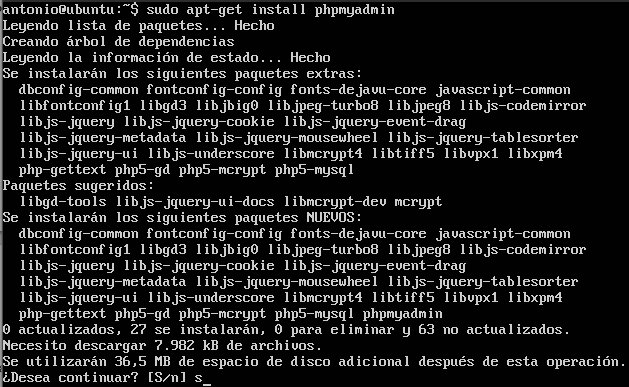
\includegraphics[scale=0.5]{imagenes/img29}
        \caption{Comando para la instalación de phpMyAdmin en Ubuntu.}
        \label{fig26}
    \end{center}
\end{figure}

\begin{figure}[H]
    \begin{center}
        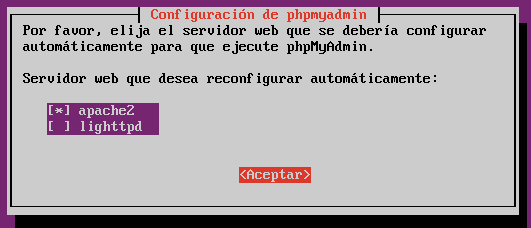
\includegraphics[scale=0.5]{imagenes/img30}
        \caption{Cuadro para seleccionar el servidor web que se quiere configurar.}
        \label{fig27}
    \end{center}
\end{figure}

\begin{figure}[H]
    \begin{center}
        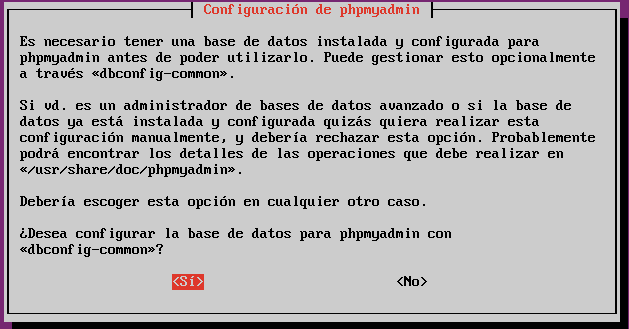
\includegraphics[scale=0.5]{imagenes/img31}
        \caption{Selección de la forma para configurar la base de datos.}
        \label{fig28}
    \end{center}
\end{figure}

\begin{figure}[H]
    \begin{center}
        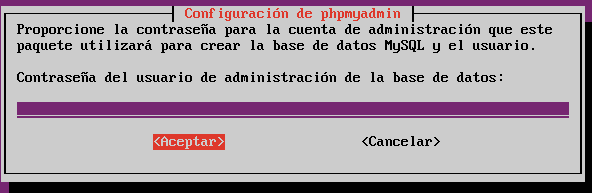
\includegraphics[scale=0.5]{imagenes/img32}
        \caption{Selección de una contraseña para el administrados de phpMyAdmin.}
        \label{fig29}
    \end{center}
\end{figure}

\begin{figure}[H]
    \begin{center}
        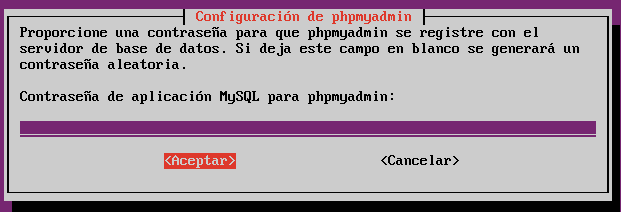
\includegraphics[scale=0.5]{imagenes/img33}
        \caption{Selección de una contraseña para que phpMyAdmin se registre en el servidor de bases de datos.}
        \label{fig30}
    \end{center}
\end{figure}

\begin{figure}[H]
    \begin{center}
        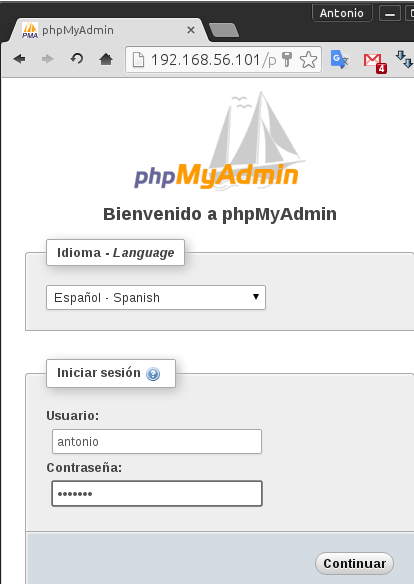
\includegraphics[scale=0.4]{imagenes/img34}
        \caption{Acceso a phpMyAdmin para probar su correcto funcionamiento.}
        \label{fig31}
    \end{center}
\end{figure}


En mi caso el tamaño límite de importación es de 2 MB ( aunque \texttt{post\_max\_size} es 8MB ) como se puede ver en la figura \ref{fig32}. Para modificar este límite, debemos editar la configuración de PHP, para ello debemos abrir el archivo php.ini localizado en /etc/php5/apache2/php.ini , ya que estamos usando Apache como servidor web para phpMyAdmin, y editar las variables \texttt{upload\_max\_filesize} que indica el tamaño máximo que puede tener el archivo que se va a subir \cite{php} y  \texttt{post\_max\_size } que indica el tamaño maximo de datos de POST permitido \cite{php1} ( este tamaño debe ser superior al de \texttt{upload\_max\_filesize}) , indicando el nuevo tamaño máximo para la importación, como se puede ver en las figuras \ref{fig33} y \ref{fig34}. Tras realizar esto y reiniciar Apache ( \texttt{service apache2 restart} ) podemos observar ( figura \ref{fig35} ) que el nuevo tamaño máximo es el indicado en \texttt{upload\_max\_filesize}.

\begin{figure}[H]
    \begin{center}
        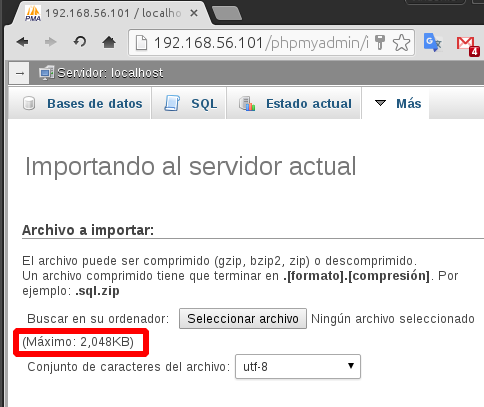
\includegraphics[scale=0.5]{imagenes/img35}
        \caption{Tamaño máximo de importación original.}
        \label{fig32}
    \end{center}
\end{figure}

\begin{figure}[H]
    \begin{center}
        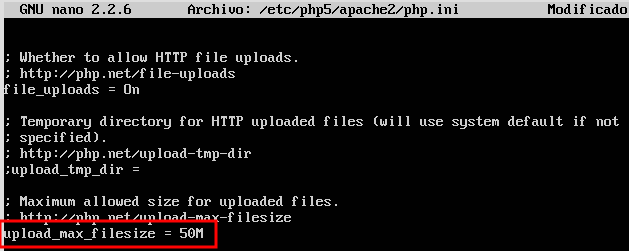
\includegraphics[scale=0.5]{imagenes/img36}
        \caption{Modificación de \texttt{upload\_max\_filesize}.}
        \label{fig33}
    \end{center}
\end{figure}

\begin{figure}[H]
    \begin{center}
        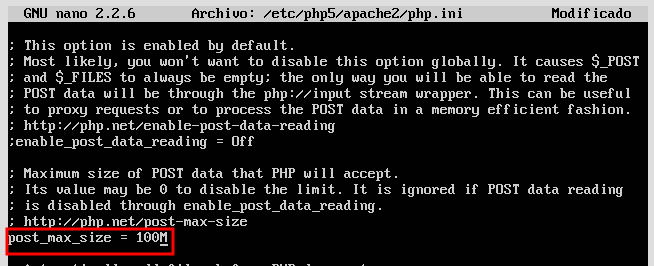
\includegraphics[scale=0.5]{imagenes/img37}
        \caption{Modificación de \texttt{post\_max\_size}.}
        \label{fig34}
    \end{center}
\end{figure}

\begin{figure}[H]
    \begin{center}
        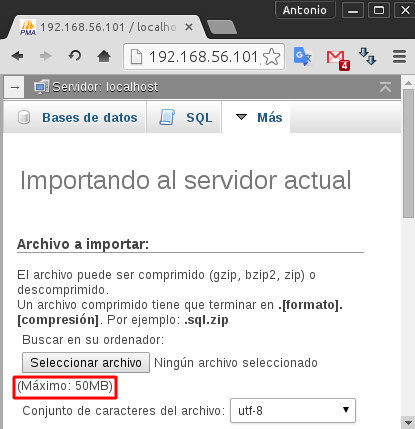
\includegraphics[scale=0.5]{imagenes/img38}
        \caption{Nuevo tamaño máximo de importación.}
        \label{fig35}
    \end{center}
\end{figure}

\subsection{Más administradores:ISPCONFIG, DIRECTADMIN, CPANEL, PARALLELS PLESK,... }
%***********************************************
%    CUESTIÓN 16
%***********************************************
\subsubsection{Cuestión 16}
\textit{Viste al menos una de las webs de los software mencionados y pruebe las demos que ofrecen realizando capturas de pantalla y comentando qué está realizando.}
\newline

En esta cuestión he usado la demo de Parallels Plesk , disponible en \cite{pp}. Desde la pantalla inicial de Parallels Plesk \ref{fig51}, me he dirigido al apartado de configuración de FTP \ref{fig52}, una vez ahí, he creado un nuevo usuario para FTP mediante el formulario mostrado en la figura \ref{fig53}, una vez rellenado se crea el usuario, sin necesidad de realizar nada mas. Como se puede ver en la figura \ref{fig54}, el usuario ahora ya aparece en la lista de los usuarios de FTP.

\begin{figure}[H]
    \begin{center}
        \advance\leftskip-2.2cm
        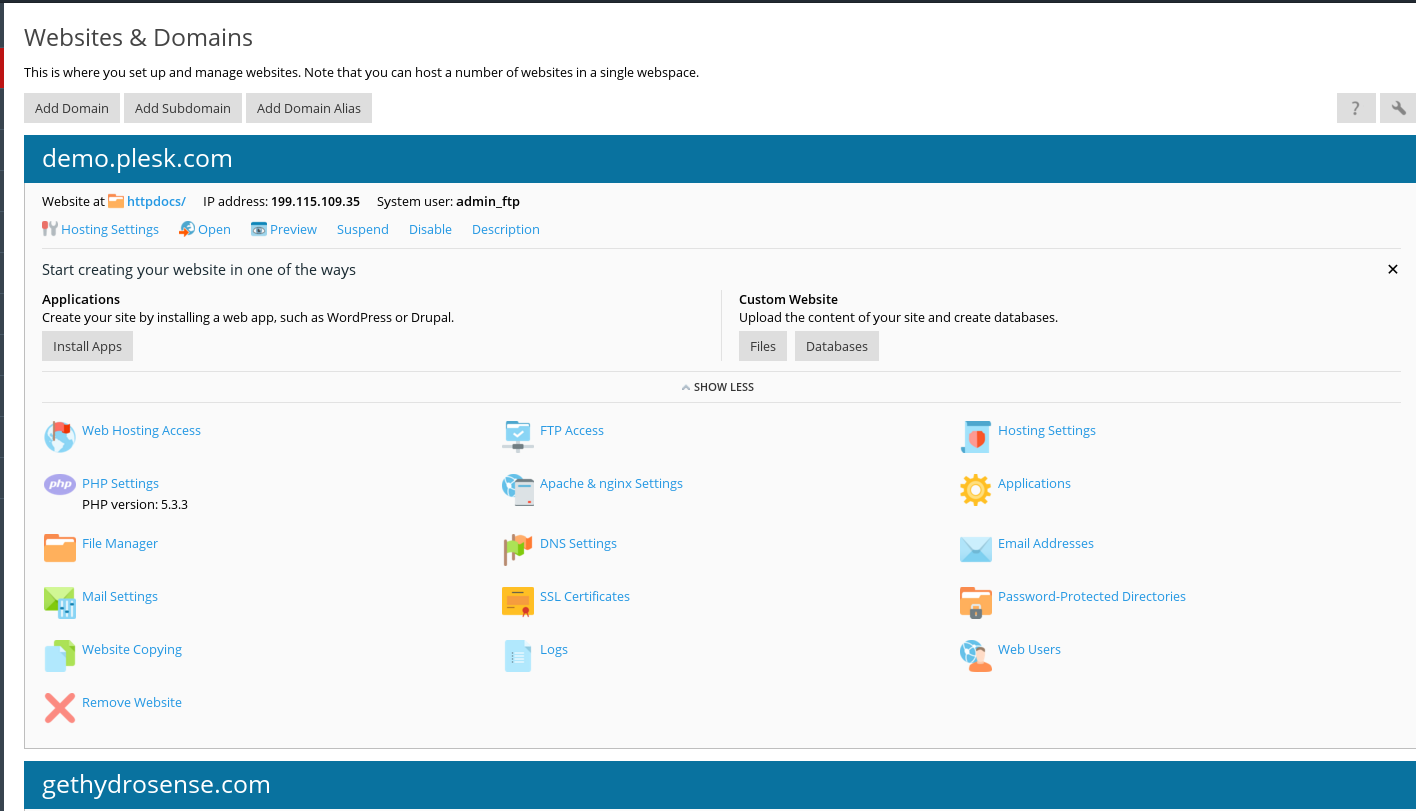
\includegraphics[scale=0.35]{imagenes/img56}
        \caption{Pagina inicial de Parallels Plesk.}
        \label{fig51}
    \end{center}
\end{figure}

\begin{figure}[H]
    \begin{center}
        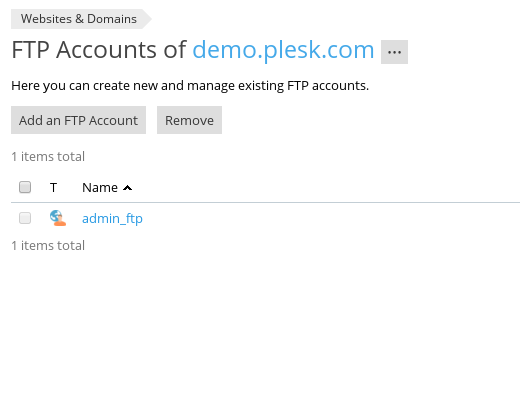
\includegraphics[scale=0.5]{imagenes/img57}
        \caption{Panel de configuración de usuarios de FTP.}
        \label{fig52}
    \end{center}
\end{figure}

\begin{figure}[H]
    \begin{center}
        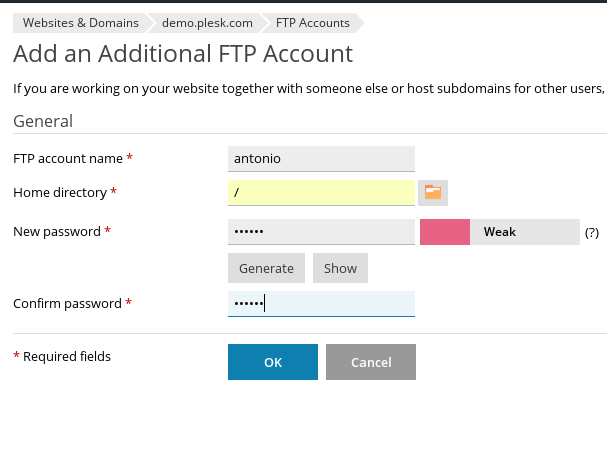
\includegraphics[scale=0.5]{imagenes/img58}
        \caption{Formulario para crear un nuevo usuario.}
        \label{fig53}
    \end{center}
\end{figure}

\begin{figure}[H]
    \begin{center}
        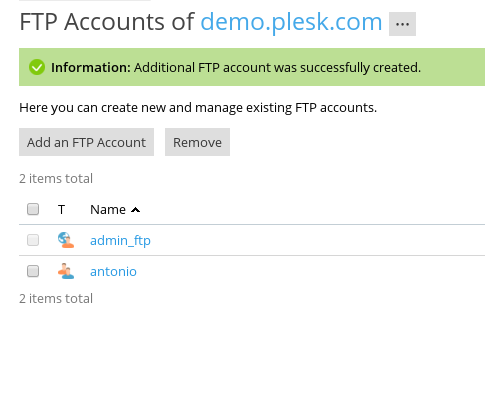
\includegraphics[scale=0.5]{imagenes/img59}
        \caption{Panel de configuración con el nuevo usuario.}
        \label{fig54}
    \end{center}
\end{figure}




\section{Automatización de tareas con scripts}
\subsection{Shells}
%***********************************************
%    CUESTIÓN 17
%***********************************************
\subsubsection{Cuestión 17}
\textit{Ejecute los ejemplos de find, grep y escriba el script que haga uso de sed para cambiar la configuración de ssh y reiniciar el servicio.}
\newline

La ejecución del ejemplo de grep ( \texttt{grep -Af | firefox} ) muestra la información sobre el proceso firefox en formato completo como muestra en la figura \ref{fig42}. La ejecución del comando \texttt{find ~/Documentos -name '*pdf' -exec cp {} ~/PDFs \;} busca los pdf que hay en Documentos y cada vez que encuentra uno, ejecuta cp y lo copia al directorio PDFs, en las figuras \ref{fig43}, \ref{fig44} y \ref{fig45} , se puede ver el funcionamiento de la orden.

\begin{figure}[H]
    \begin{center}
        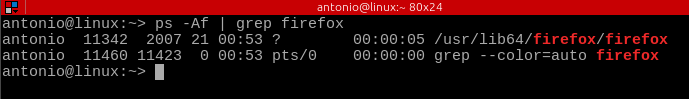
\includegraphics[scale=0.6]{imagenes/img45}
        \caption{Ejecución de la orden \texttt{grep -Af | firefox}.}
        \label{fig42}
    \end{center}
\end{figure}

\begin{figure}[H]
    \begin{center}
        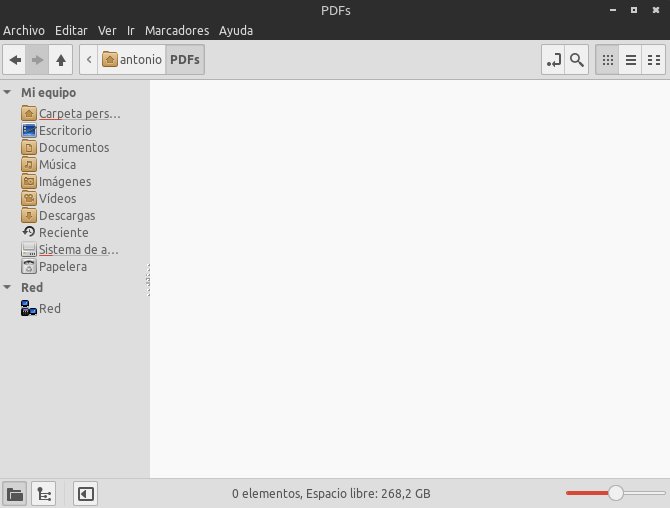
\includegraphics[scale=0.5]{imagenes/img46}
        \caption{Estado de la carpeta PDFs antes de la ejecución de la orden.}
        \label{fig43}
    \end{center}
\end{figure}

\begin{figure}[H]
    \begin{center}
        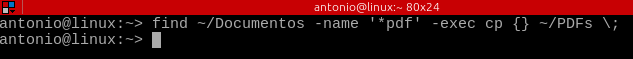
\includegraphics[scale=0.6]{imagenes/img47}
        \caption{Ejecución de la orden  \texttt{find ~/Documentos -name '*pdf' -exec cp {} ~/PDFs \;}. }
        \label{fig44}
    \end{center}
\end{figure}

\begin{figure}[H]
    \begin{center}
        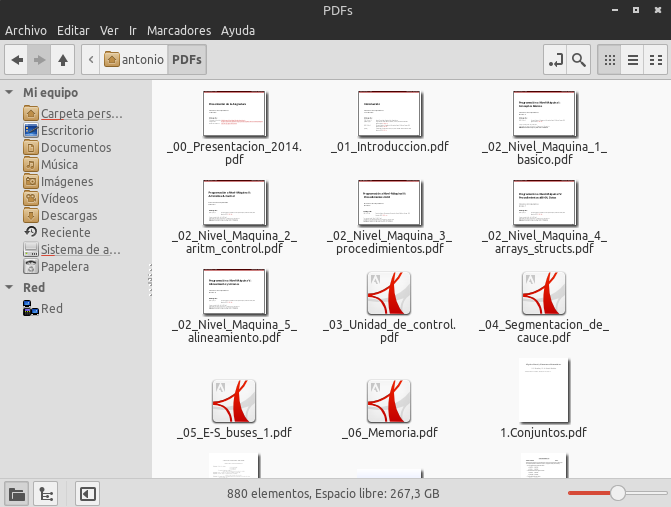
\includegraphics[scale=0.5]{imagenes/img48}
        \caption{Estado de la carpeta PDFs después de la ejecución de la orden.}
        \label{fig45}
    \end{center}
\end{figure}


Para probar sed he creado un script que pide un nuevo puerto para SSH y cambia la configuración del puerto de SSH durante 60 segundos, luego vuelve a poner SSH en el puerto 22, como se puede ver en las figuras \ref{fig46}, \ref{fig47} y \ref{fig48}.\cite{sed}


\begin{figure}[H]
    \begin{center}
        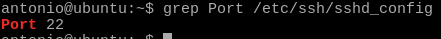
\includegraphics[scale=0.8]{imagenes/img49}
        \caption{Configuración original del puerto de SSH.}
        \label{fig46}
    \end{center}
\end{figure}

\begin{figure}[H]
    \begin{center}
        \advance\leftskip-2cm
        \includegraphics[scale=0.65]{imagenes/img50}
        \caption{Código del script usado para la prueba de sed.}
        \label{fig47}
    \end{center}
\end{figure}


\begin{figure}[H]
    \centering
    \begin{subfigure}[b]{0.72\textwidth}
        \includegraphics[width=\textwidth]{imagenes/img51}
        \caption{Ejecución del script.} 
    \end{subfigure}
   \begin{subfigure}[b]{0.8\textwidth}
        \includegraphics[width=\textwidth]{imagenes/img52}
        \caption{Muestra del nuevo puerto en la configuración de SSH.} 
    \end{subfigure}
    \begin{subfigure}[b]{0.8\textwidth}
        \includegraphics[width=\textwidth]{imagenes/img53}
        \caption{Prueba de conexión SSH con el nuevo puerto.} 
    \end{subfigure}
    \caption{Prueba del script.}  
    \label{fig48} 
\end{figure}
%***********************************************
%    CUESTIÓN OP6
%***********************************************
\subsubsection{Cuestión opcional 6}
\textit{Muestre un ejemplo de uso para awk.}
\newline

Para probar el comando awk, he creado un programa ( figura \ref{fig36} ) de awk que cuenta cuantos números hay que ocupen la tercera posición en una línea en la que los que los elementos están separados por espacios y además realiza la suma de estos elementos. Para probar el programa he usado un archivo como el de la figura \ref{fig37}, con el que se obtiene el resultado mostrado en la figura \ref{fig38}.Para la realización de este programa me he ayudado del manual disponible en \cite{awk}


\begin{figure}[H]
    \begin{center}
    \advance\leftskip-2.2cm
        \includegraphics[scale=0.75]{imagenes/img39}
        \caption{Programa de AWK.}
        \label{fig36}
    \end{center}
\end{figure}

\begin{figure}[H]
    \begin{center}
        \includegraphics[scale=0.8]{imagenes/img40}
        \caption{Archivo que se le pasa al programa.}
        \label{fig37}
    \end{center}
\end{figure}

\begin{figure}[H]
    \begin{center}
    \advance\leftskip-1cm
        \includegraphics[scale=0.7]{imagenes/img41}
        \caption{Ejecución del programa sobre el archivo.}
        \label{fig38}
    \end{center}
\end{figure}




\subsection{PHP}
\subsection{Python}
%***********************************************
%    CUESTIÓN 18
%***********************************************
\subsubsection{Cuestión 18}
\textit{Escriba el script para cambiar el acceso a ssh usando PHP o Python.}
\newline

Para este ejercicio he realizado un script en Python que hace modifica la configuración de SSH de modo que permita o no hacer login desde la cuenta de usuario root y luego reinicia el servicio \cite{subp} en la figura \ref{fig49} se puede ver el código y en la figura \ref{fig50}, se puede ver una prueba de la ejecución. 

\begin{figure}[H]
    \begin{center}
    \advance\leftskip-1cm
        \includegraphics[scale=0.5]{imagenes/img54}
        \caption{Código del script en Python.}
        \label{fig49}
    \end{center}
\end{figure}

\begin{figure}[H]
    \begin{center}
    \advance\leftskip-1cm
        \includegraphics[scale=0.5]{imagenes/img55}
        \caption{Prueba de la ejecución del script.}
        \label{fig50}
    \end{center}
\end{figure}

Otro ejemplo de script en python es el mostrado en la figura \ref{py}, que muestra una interesante capacidad de python, la de llamar a un script de bash. Gracias a esto, podemos reutilizar código, y con una sola linea, obtenemos un script en python, que permite modificar los puertos de SSH haciendo uso del script mostrado en la figura \ref{fig47}. El resultado de la ejecución de este script es exactamente igual que el del script de bash mostrado en la cuestión 17 (figura \ref{py2}). 
\begin{figure}[H]
    \begin{center}
    \advance\leftskip-1cm
        \includegraphics[scale=0.75]{imagenes/py}
        \caption{Script de python que llama al script de la figura \ref{fig47}. ( Cambia el puerto de SSH durante 60 segundos y luego vuelve a poner el puerto 22).}
        \label{py}
    \end{center}
\end{figure}

\begin{figure}[H]
    \begin{center}
        \includegraphics[scale=0.75]{imagenes/py2}
        \caption{Ejecución del script de python.}
        \label{py2}
    \end{center}
\end{figure}

\subsection{Windows PowerShell}
%***********************************************
%    CUESTIÓN 19
%***********************************************
\subsubsection{Cuestión 19}
\textit{Abra una consola de Powershell y pruebe a parar un programa en ejecución (p.ej), realice capturas de pantalla y comente lo que muestra.}
\newline

Para realizar esta prueba en primer lugar he abierto Internet Explorer, luego en PowerShell he ejecutado la orden \texttt{Get-Process} \cite{gpps} ( figura \ref{fig39} ) para obtener el nombre del proceso y por último he ejecutado la orden \texttt{Stop-Porcess} \cite{spps} para detener el proceso (figura \ref{fig39}). En lugar de usar la opción \texttt{-Name}, se podría haber detenido el proceso haciendo uso de su Id. 

\begin{figure}[H]
    \begin{center}
    \advance\leftskip-1cm
        \includegraphics[scale=0.7]{imagenes/img42}
        \caption{Ejecución orden \texttt{Get-Process} en PowerShell.}
        \label{fig39}
    \end{center}
\end{figure}

\begin{figure}[H]
    \begin{center}
    \advance\leftskip-1cm
        \includegraphics[scale=0.7]{imagenes/img43}
        \caption{Ejecución orden \texttt{Stop-Porcess -Name} en PowerShell.}
        \label{fig40}
    \end{center}
\end{figure}

%*************************************************************
\newpage
\bibliographystyle{ieeetr}
\bibliography{citas}

\end{document}
